%%
%% Copyright 2007, 2008, 2009 Elsevier Ltd
%%
%% This file is part of the 'Elsarticle Bundle'.
%% ---------------------------------------------
%%
%% It may be distributed under the conditions of the LaTeX Project Public
%% License, either version 1.2 of this license or (at your option) any
%% later version.  The latest version of this license is in
%%    http://www.latex-project.org/lppl.txt
%% and version 1.2 or later is part of all distributions of LaTeX
%% version 1999/12/01 or later.
%%
%% The list of all files belonging to the 'Elsarticle Bundle' is
%% given in the file `manifest.txt'.
%%

%% Template article for Elsevier's document class `elsarticle'
%% with numbered style bibliographic references
%% SP 2008/03/01
%%
%%
%%
%% $Id: elsarticle-template-num.tex 4 2009-10-24 08:22:58Z rishi $
%%
%%

%\documentclass[preprint,12pt]{elsarticle}

%% Use the option review to obtain double line spacing
%% \documentclass[preprint,review,12pt]{elsarticle}

%% Use the options 1p,twocolumn; 3p; 3p,twocolumn; 5p; or 5p,twocolumn
%% for a journal layout:
%% \documentclass[final,1p,times]{elsarticle}
%% \documentclass[final,1p,times,twocolumn]{elsarticle}
%% \documentclass[final,3p,times]{elsarticle}
%% \documentclass[final,3p,times,twocolumn]{elsarticle}
%% \documentclass[final,5p,times]{elsarticle}
\documentclass[final,5p,times,twocolumn]{elsarticle}

%% if you use PostScript figures in your article
%% use the graphics package for simple commands
%% \usepackage{graphics}
%% or use the graphicx package for more complicated commands
\usepackage{graphicx}
%% or use the epsfig package if you prefer to use the old commands
%% \usepackage{epsfig}

%% The amssymb package provides various useful mathematical symbols
\usepackage{amssymb}
%% The amsthm package provides extended theorem environments
%% \usepackage{amsthm}

%% The lineno packages adds line numbers. Start line numbering with
%% \begin{linenumbers}, end it with \end{linenumbers}. Or switch it on
%% for the whole article with \linenumbers after \end{frontmatter}.
%% \usepackage{lineno}

%% natbib.sty is loaded by default. However, natbib options can be
%% provided with \biboptions{...} command. Following options are
%% valid:

%%   round  -  round parentheses are used (default)
%%   square -  square brackets are used   [option]
%%   curly  -  curly braces are used      {option}
%%   angle  -  angle brackets are used    <option>
%%   semicolon  -  multiple citations separated by semi-colon
%%   colon  - same as semicolon, an earlier confusion
%%   comma  -  separated by comma
%%   numbers-  selects numerical citations
%%   super  -  numerical citations as superscripts
%%   sort   -  sorts multiple citations according to order in ref. list
%%   sort&compress   -  like sort, but also compresses numerical citations
%%   compress - compresses without sorting
%%
%% \biboptions{comma,round}

% \biboptions{}


\journal{Journal of Chromatography B}

\begin{document}

\begin{frontmatter}

%% Title, authors and addresses

%% use the tnoteref command within \title for footnotes;
%% use the tnotetext command for the associated footnote;
%% use the fnref command within \author or \address for footnotes;
%% use the fntext command for the associated footnote;
%% use the corref command within \author for corresponding author footnotes;
%% use the cortext command for the associated footnote;
%% use the ead command for the email address,
%% and the form \ead[url] for the home page:
%%
%% \title{Title\tnoteref{label1}}
%% \tnotetext[label1]{}
%% \author{Name\corref{cor1}\fnref{label2}}
%% \ead{email address}
%% \ead[url]{home page}
%% \fntext[label2]{}
%% \cortext[cor1]{}
%% \address{Address\fnref{label3}}
%% \fntext[label3]{}

%& SHORT COMMUNICATION about 2850 words 
\title{Straightforward interpretation of metabolomics, proteomics, transcriptomics and genomics data by comprehensive visualization and pathway enrichment using a single software tool}

%% use optional labels to link authors explicitly to addresses:
%% \author[label1,label2]{<author name>}
%% \address[label1]{<address>}
%% \address[label2]{<address>}

\author[uni]{Lars Rosenbaum\corref{cor}}
\ead{lars.rosenbaum@uni-tuebingen.de}
\author[uni]{Johannes Eichner}
\author[uni]{Clemens Wrzodek}
\author[uni]{Andreas Zell}
\author[klinikum,dzd]{Rainer Lehmann\corref{cor}}
\ead{rainer.lehmann@med.uni-tuebingen.de}
\address[uni]{Center for Bioinformatics, University of T\"ubingen, T\"ubingen, Germany}
\address[klinikum]{Division of Clinical Chemistry and Pathobiochemistry (Central Laboratory), University Hospital T\"ubingen, T\"ubingen, Germany}
\address[dzd]{Institute of Diabetes Research and Metabolic Diseases, Member of the German Center for Diabetes Research, University of T\"ubingen, T\"ubingen, Germany}
\cortext[cor]{Corresponding authors. Tel. +49-7071-29-8 31 93}

\begin{abstract}
%% Text of abstract
In systems biology, the combination of multiple types of omics data, such as metabolomics, transcriptomics, and proteomics, yields more information on a biological process than the analysis of a single type of data. Today, data from different omics platforms is usually combined in one experimental setup to obtain insight into a biological process or a disease state. Particularly high accuracy metabolomics data from modern mass spectrometry instruments is more and more integrated into biological studies. Reflecting this trend, we updated InCroMAP to allow for the integration of metabolomics data. The tool is able to perform an integrated enrichment analysis and pathway-based visualization of metabolomics, transcriptomics, and proteomics data.
\end{abstract}

\begin{keyword}
%% keywords here, in the form: keyword \sep keyword
Metabolomics \sep Transcriptomics \sep Proteomics \sep Systems biology \sep Enrichment analysis \sep Pathway visualization
%% MSC codes here, in the form: \MSC code \sep code
%% or \MSC[2008] code \sep code (2000 is the default)

\end{keyword}

\end{frontmatter}

%%
%% Start line numbering here if you want
%%
% \linenumbers

%% main text
\section{Introduction}
Today, high-throughput methods for the analysis of biological systems, such as microarrays, next generation sequencing, and mass spectrometry generate a wealth of genome-scale data. To develop hypotheses about a biological process or a disease state, a variety of omics-platforms for measuring different genomic, proteomic, and metabolic features are combined in one experimental setup. Probably the most prominent genomic feature is messenger RNA (mRNA), which can be quantified on a genome wide level by gene expression chips (microarrays) or next generation sequencing techniques. Other important (epi)genomic features include microRNA (miRNA), single-nucleotide polymorphisms, and epigenetic information, such as the promoter methylation status (DNAm). Proteomic features can be derived from abundance profiling of particular protein isoforms and post translational modifications, such as methylation and phosphorylation. Furthermore, modern mass spectrometry platforms are able to detect and measure the relative intensity of thousands of metabolites with high accuracy. The sensible and integrated visualization of omics data at different levels of abstraction is crucial to obtain biological insight without being overwhelmed by the intrinsic complexity of the data \cite{Gehlenborg2010}. A key concept for detecting alterations in cell signalling or metabolism in a biological system are pathway-based visualizations.

A plethora of tools were developed for the inspection of data from individual platforms (see \cite{Gehlenborg2010} for examples). Furthermore, solutions for the combined visualization of transcriptomics (mRNA) and metabolomics data exist \cite{Garcia-Alcalde2011,Waegele2012}. Both Paintomics \cite{Garcia-Alcalde2011} and MassTRIX \cite{Waegele2012} are web-service based tools that are able to visualize mRNA microarray and identified metabolomics data in KEGG \cite{Kanehisa2006} pathways. MassTRIX is able to handle unidentified metabolic data by comparing a mass against theoretical adducts stored in metabolomics databases. An example of a tool that can handle several heterogeneous types of omics data is the commercial Ingenuity Pathway Analysis software (www.ingenuity.com). However, Ingenuity does not provide an integrated visualization of multi-level omics data. Thus, most available high-level analysis tools are not freely available, focused on certain specialized platforms, or not able to perform an integrated analysis of many different types of heterogeneous data. However, complex interactions between multiple layers of gene regulation can only be inferred by the integration of omics datasets across multiple platforms, which requires novel analysis tools with appropriate visualizations.

In this contribution we present an extended version of InCroMAP \cite{Wrzodek2012a,Wrzodek2012b}. Up to the present, InCroMAP is a stand-alone Java software which provides an enrichment analysis and pathway-based visualizations of genomic and proteomic data, where multiple biological layers were monitored in the same set of samples. The current version supports the integrated analysis of heterogeneous genomic and epigenomic features, such as mRNA, miRNA, and DNAm, as well as abundance profiles of post translational protein modifications. Furthermore, InCroMAP can import data from any platform which contains expression values that can be either associated to a certain gene or a genomic region. The application was developed to provide a high ease of use. Consequently, all information required, for example, for the mapping between different feature identifiers or the annotation of miRNAs with mRNA targets, is either directly included in the tool or dynamically downloaded in the background. However, up to now the application has not been able to process metabolomics data. Thus, in the extended version of InCroMAP, we also support the enrichment analysis and pathway-based visualization of annotated metabolomics data. The tool can import data annotated with specific metabolic database identifiers (e.g. HMDB \cite{Wishart2009}) or automatically recognize common compound names or IUPAC names.

InCroMAP is freely available under the LGPL3 license at http://www.cogsys.cs.uni-tuebingen.de/software/InCroMAP, including a comprehensive user’s guide and several example data files to test the capabilities of the tool.

\section{Methods}
Before systems biology data from heterogeneous platforms can be integrated and visualized with high-level data analysis tools like InCroMAP, the data has to be processed with platform dependent workflows (see Figure \ref{fig:incromap-workflow}). A typical workflow for metabolomics data from untargeted mass spectrometry measurements includes the following steps. First, metabolic features, which are characterized by mass and relative intensity, are extracted from the raw data files with feature finding and feature extraction algorithms. Optimally, the feature induced by a metabolite should contain all signals that were generated by the metabolite. Second, the extracted features have to be aligned and linked between the different samples. The aforementioned preprocessing steps can be performed with sophisticated open-source software tools like OpenMS \cite{Sturm2008}. The  features are then subjected to quality controls and low-level statistical data analysis, which includes normalization and calculation of measures for differential intensities between conditions (e.g. p-values from some statistical model, fold changes, or log ratios). Mostly, these tasks are performed with commercial statistics software, open-source omics analysis applications like Mayday \cite{Battke2010}, or directly with the statistical programming language R (www.r-project.org). In a final preprocessing step, the metabolite features are annotated with candidate identifiers using information provided by metabolomics databases, such as PubChem \cite{Wang2009}, HMDB \cite{Wishart2009}, or LIPID MAPS \cite{Sud2007}. Similar preprocessing workflows exist for other platforms, like microarrays and next generation sequencing. The processed data can then be imported and analyzed with InCroMAP.

In a typical use case of InCroMAP (see Figure \ref{fig:incromap-workflow}), the user first imports his preprocessed multi-level omics data, given in tabular format. Then, the differentially expressed metabolites or genes for each platform are determined based on appropriate cutoffs and relevant pathways related to the system biological background of the experiments are inferred. For the detection of relevant pathways, InCroMAP employs a special pathway enrichment algorithm which integrates differentially expressed metabolites and genes across multiple platforms. The resulting pathways can then be selected for further visual inspection from a table in which each pathway is associated with a significance value. Alternatively, the metabolic overview function of InCroMAP can be used to generate an interactive global map of cellular metabolism, in which each subordinate metabolic pathway is colored according to the significance of its enrichment. The results of the enrichment analysis can be exported in tabular format and the pathway-based visualizations can be easily stored as JPEG images.

\begin{figure*}
\center
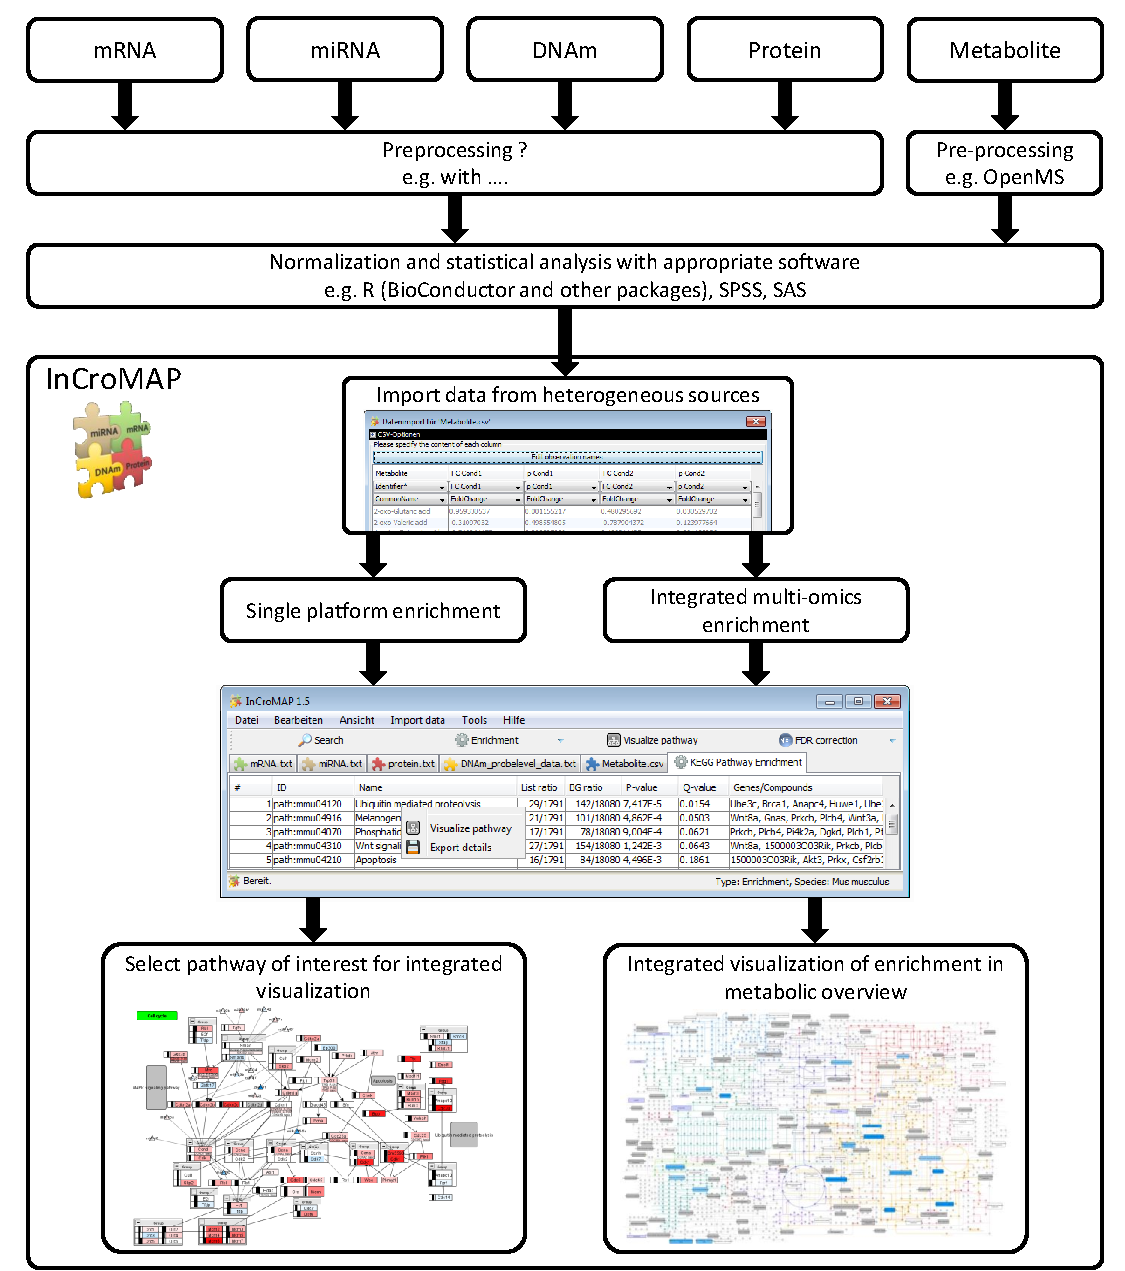
\includegraphics[width=0.9\textwidth]{InCroMAP_workflow.pdf}
\caption{The flow chart depicts the general workflow for performing an analysis with InCroMAP. Each data type is preprocessed (e.g. feature detection, feature extraction) using a appropriate, platform dependent tool. Then, the data is normalized and statistically analyzed with a statistics software, which yields p-values or fold changes for each of the features. Finally, the gene and metabolite features are annotated with candidate identifiers. After these preprocessing steps the data can be easily importet to InCroMAP and an enrichment analysis can be performed. From the enrichment, a user can choose to visualize the information of all platforms in a chosen pathway or to generate a metabolic overview to identify alterations in metabolic pathways.}
\label{fig:incromap-workflow}
\end{figure*}

\begin{figure*}[t]
\center
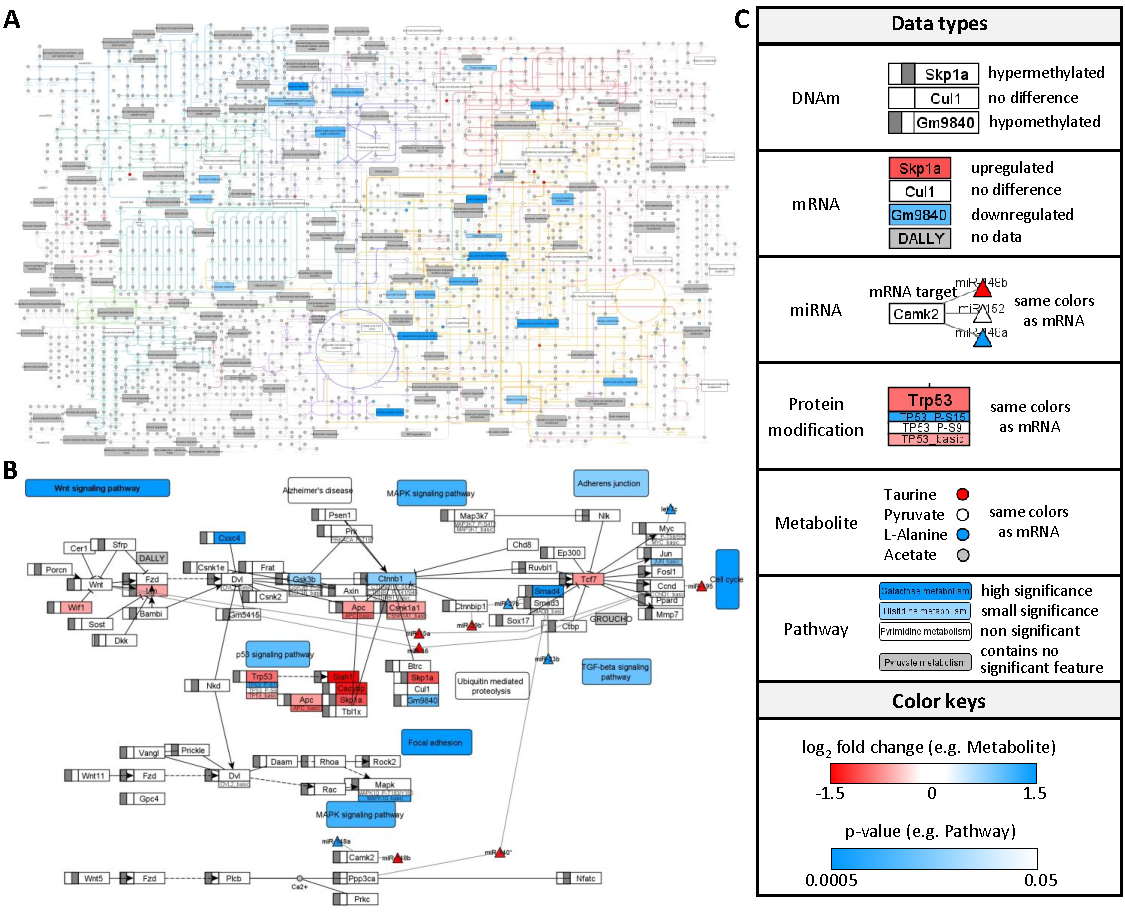
\includegraphics[width=1.0\textwidth]{InCroMAP_examples.pdf}
\caption{(A) shows the metabolic overview with visualized metabolic data and pathway enrichment p-values. (B) shows the Wnt signaling pathway with visualized data from all supported platforms. Both visualizations were generated with the example data provided on the project web page.}
\label{fig:incromap-examples}
\end{figure*}

%%POSSIBLY INCLUDE ALL SUBSECTION JUST IN METHODS SECTION TO SAVE SPACE

\subsection{Data import}
For an import to InCroMAP the data has to be in a tabular format, which can be easily obtained by MS Excel export functions. Furthermore, each measurement must contain at least some identifier and an observation (p-value, fold-change, or log ratio) that captures the difference between experimental conditions. InCroMAP is able to handle various types of identifiers for transcriptomics, proteomics, and metabolomics data. It supports the automatic recognition of identifiers used by the most common oligonucleotide microarray manufacturers (e.g., Affymetrix, Agilent, etc.) and generic formats to enable the import of processed data, provided that each measurement can be either associated to a certain gene, genomic region, or metabolite. Metabolomics data may be annotated by a database identifier (e.g. KEGG, HMDB, PubChem, LIPID MAPS) or by a common synonym or IUPAC name.

\subsection{Enrichment analysis}
A common algorithm for performing an enrichment of gene sets is an overrepresentation analysis \cite{Backes2007}, which uses a hypergeometric test to calculate a significance value for each predefined gene set. InCroMAP extends the method to provide an integral enrichment over multiple platforms. The overrepresentation analysis requires a fixed set of up- or downregulated genes or metabolites, which are obtained by a user defined fold-change and/or p-value cutoff for each of the platform dependent data sets. Currently, InCroMAP supports the enrichment of KEGG pathways, of gene sets from the molecular signatures database (MSigDB), and of gene ontology (GO) terms. The result of a KEGG pathway enrichment is depicted in Figure \ref{fig:incromap-workflow}, where each pathway is assigned a p-value and an FDR corrected p-value (q-value).

\subsection{Metabolic overview}
TODO JOHANNES
Visualization as compound nodes with potential names
common name automatically assigned to each node

\subsection{Pathway-based visualization}
TODO JOHANNES
Being rendered in an interactive graph viewer, the pathway nodes (i.e., genes) can be overlaid with expression data from mRNAs and multiple protein products. Additionally, miRNAs can be connected to a given pathway based on experimentally confirmed or predicted interactions to their target mRNAs. If desired, the tool also visualizes differential methylation of proximal gene promoters, which is by default computed based on the largest peak observed in the upstream region of the transcription start site.

Furthermore: Pathways of interest can then either be automatically downloaded from KEGG or imported from other sources in BioPAX format. 

\section{Results and discussion}
We presented an extended version of InCroMAP, which allows the integrated pathway-based visualization of data from multiple omics platforms, such as metabolome data, mRNA, miRNA, protein modifications, and DNAm. The tool enables a user to interactively browse through and visualize different KEGG pathways. Furthermore, the metabolic overview function of InCroMAP can be used to generate an interactive global map of cellular metabolism, which helps to identify interesting metabolic pathways. Thus, the tool provides an userful overview of multi-omics data in the context of metabolic and signalling pathways, which enables the generation of initial biological hypotheses. 

The ability to handle metabolimics data results in limitations of the current pathway enrichment method. The annotation of untargeted metabolomics data sets usually results in many-to-many mappings because a metabolic feature can be mapped to several candidate identifiers and vice versa. The overrepresentation analysis is not designed to handle such many-to-many mappings. Solutions to this problem in the setting of gene set enrichment have been proposed \cite{Kankainen2011} and will be implemented in InCroMAP. 

Further future improvements concern the integration of visualizations from additional metabolomic and lipidomics databases, such as Reactome \cite{Eustachio2011} and LIPID MAPS \cite{Sud2007}. Particularly, the inclusion of visualizations based on LIPID MAPS pathways can overcome limitations of KEGG with respect to lipidomics data. Additionally, an automatic annotation with candidate identifiers for untargeted metabolomics data based on the comparison against theoretical adducts of metabolites from metabolomic databases is planned for a future release of InCroMAP.

\section{Acknowledgements}
This project was supported by the Competence Network for Diabetes mellitus funded
by the BMBF (FKZ 01GI0803-04) and a grant from to the German Center for Diabetes Research (DZD eV). Furthermore, the project received funding from the Innovative Medicine Initiative Joint Undertaking (IMI JU) [115001] (MARCAR project).

%% The Appendices part is started with the command \appendix;
%% appendix sections are then done as normal sections
%% \appendix

%% \section{}
%% \label{}

%% References
%%
%% Following citation commands can be used in the body text:
%% Usage of \cite is as follows:
%%   \cite{key}         ==>>  [#]
%%   \cite[chap. 2]{key} ==>> [#, chap. 2]
%%

%% References with bibTeX database:


\bibliographystyle{elsarticle-num}
\bibliography{literature}

%% Authors are advised to submit their bibtex database files. They are
%% requested to list a bibtex style file in the manuscript if they do
%% not want to use elsarticle-num.bst.

%% References without bibTeX database:

% \begin{thebibliography}{00}

%% \bibitem must have the following form:
%%   \bibitem{key}...
%%

% \bibitem{}

% \end{thebibliography}


\end{document}

%%
%% End of file `elsarticle-template-num.tex'.
